\documentclass{article}
\usepackage[utf8]{inputenc}
\usepackage{amsmath}
\usepackage{amssymb}
\usepackage{indentfirst}
\usepackage{color}
\usepackage{forest}
\usepackage{fancyhdr}
\usepackage{algorithm}
\usepackage{bm}
\usepackage[noend]{algpseudocode}
\usepackage{geometry}
\usepackage[T1]{fontenc}
\geometry{left=2.5cm,right=2.5cm,top=2.5cm,bottom=2.5cm}

\title{6.046/18.410 Problem Set 9}
\author{Yijun Jiang\vspace{3pt}\\Collaborator: Hengyun Zhou, Eric Lau}
%\email{yjjiang@mit.edu}
\date{\today}

\pagestyle{fancy}
\lhead{Yijun Jiang}
\rhead{6.046/18.410 Problem Set 9}

\begin{document}
\maketitle

\section{Balancing Network}
\subsection{Part (a)}
\noindent\textbf{Proof}:
By induction. In the base case, $d=1$ and $n=2$. Send the first token through some input wire $x$. Since $d=1$, wire $x$ can input to at most one balancer. If wire $x$ inputs to a balancer $b$, the first token flips $b$. Sending the second token through the same wire flips $b$ back to its original state. So the entire network $B$ returns to its original state. If wire $x$ does not input to any balancer, sending two tokens through does not alter the state of $B$. In conclusion, the base case holds.

Now suppose the statement is true for $d=d_0$ and $n=2^{d_0}$. Consider a network $B$ with depth $d=d_0+1$ and input $n=2^{d_0+1}=2\times 2^{d_0}$ tokens through wire $x$. We can decompose $B$ into the first $d_0$ layers $B_0$ and the last layer $\Delta B$. We input $n$ tokens through wire $x$ to $B_0$ and get outputs $y_1,y_2,\cdots,y_m$. Then if we take $y_1,y_2,\cdots,y_m$ as inputs to the $m$ wires of $\Delta B$, we will get the same outputs as we directly input $n$ tokens through wire $x$ to $B$.

Divide the input tokens into two groups, each of size $2^{d_0}$. First input the first group through wire $x$ to $B_0$. By induction hypothesis, since $B_0$ has depth $d_0$, its state is recovered after all tokens in the first group have left. Therefore, inputing the second group through wire $x$ to $B_0$ generates the same outputs and also recovers $B_0$. Combining the two runs, each output wire of $B_0$ has an even number of tokens.

Then we input these tokens to $\Delta B$. Each balancer in this depth-one network receives an even number of tokens and is thus flipped an even number of times. Therefore, each balancer returns to its original state after all tokens have left. So $\Delta B$ is recovered to its original state.

Putting $B_0$ and $\Delta B$ together as a larger network $B$ of depth $d_0+1$, after $n=2^{d_0+1}$ tokens are input through wire $x$ and leave, $B$ returns to its original state.

By induction, the statement is true. If $n=2^d$ tokens enter a network of depth $d$ on the same wire and exit the network, the network will return to its original state.

\subsection{Part (b)}
\noindent\textbf{Proof}:
Let $x_{\min}=a$ be the smallest element in $X$. Then since $|x_i-x_{\min}|\leqslant k$ for all $i$, we have $a\leqslant x_i\leqslant a+k$. Similarly, let $y_{\min}=b$, we have $b\leqslant y_i\leqslant b+k$ for all $i$.

WLOG, let the one-to-one correspondence be $(x_i,y_i)$ for all $i$. According to the balancer property, the two outputs, denoted by $z_i^\alpha$ where $\alpha=1,2$, satisfy
\begin{equation*}
\left\lfloor\frac{x_i+y_i}{2}\right\rfloor\leqslant z_i^\alpha\leqslant\left\lceil\frac{x_i+y_i}{2}\right\rceil
\end{equation*}

Therefore, for all $i$ and $\alpha$,
\begin{equation*}
\left\lfloor\frac{a+b}{2}\right\rfloor\leqslant z_i^\alpha\leqslant\left\lceil\frac{a+b}{2}\right\rceil+k
\end{equation*}

For any two elements in $Z$, we have
\begin{equation*}
|z_i^\alpha-z_j^\beta|\leqslant\left\lceil\frac{a+b}{2}\right\rceil+k-\left\lfloor\frac{a+b}{2}\right\rfloor\leqslant k+1
\end{equation*}

This means that $Z$ is $(k+1)$-smooth.

\section{OddEven Network}
\subsection{Part (a)}
If we input three tokens through wire 1 of an OddEven(4) network, two tokens will end up on output wire 1 and one token on output wire 2. The output does not have step property. Therefore, OddEven(4) is not a counting network. See Figure \ref{oddeven}.
\begin{figure}[!htbp]
\centering
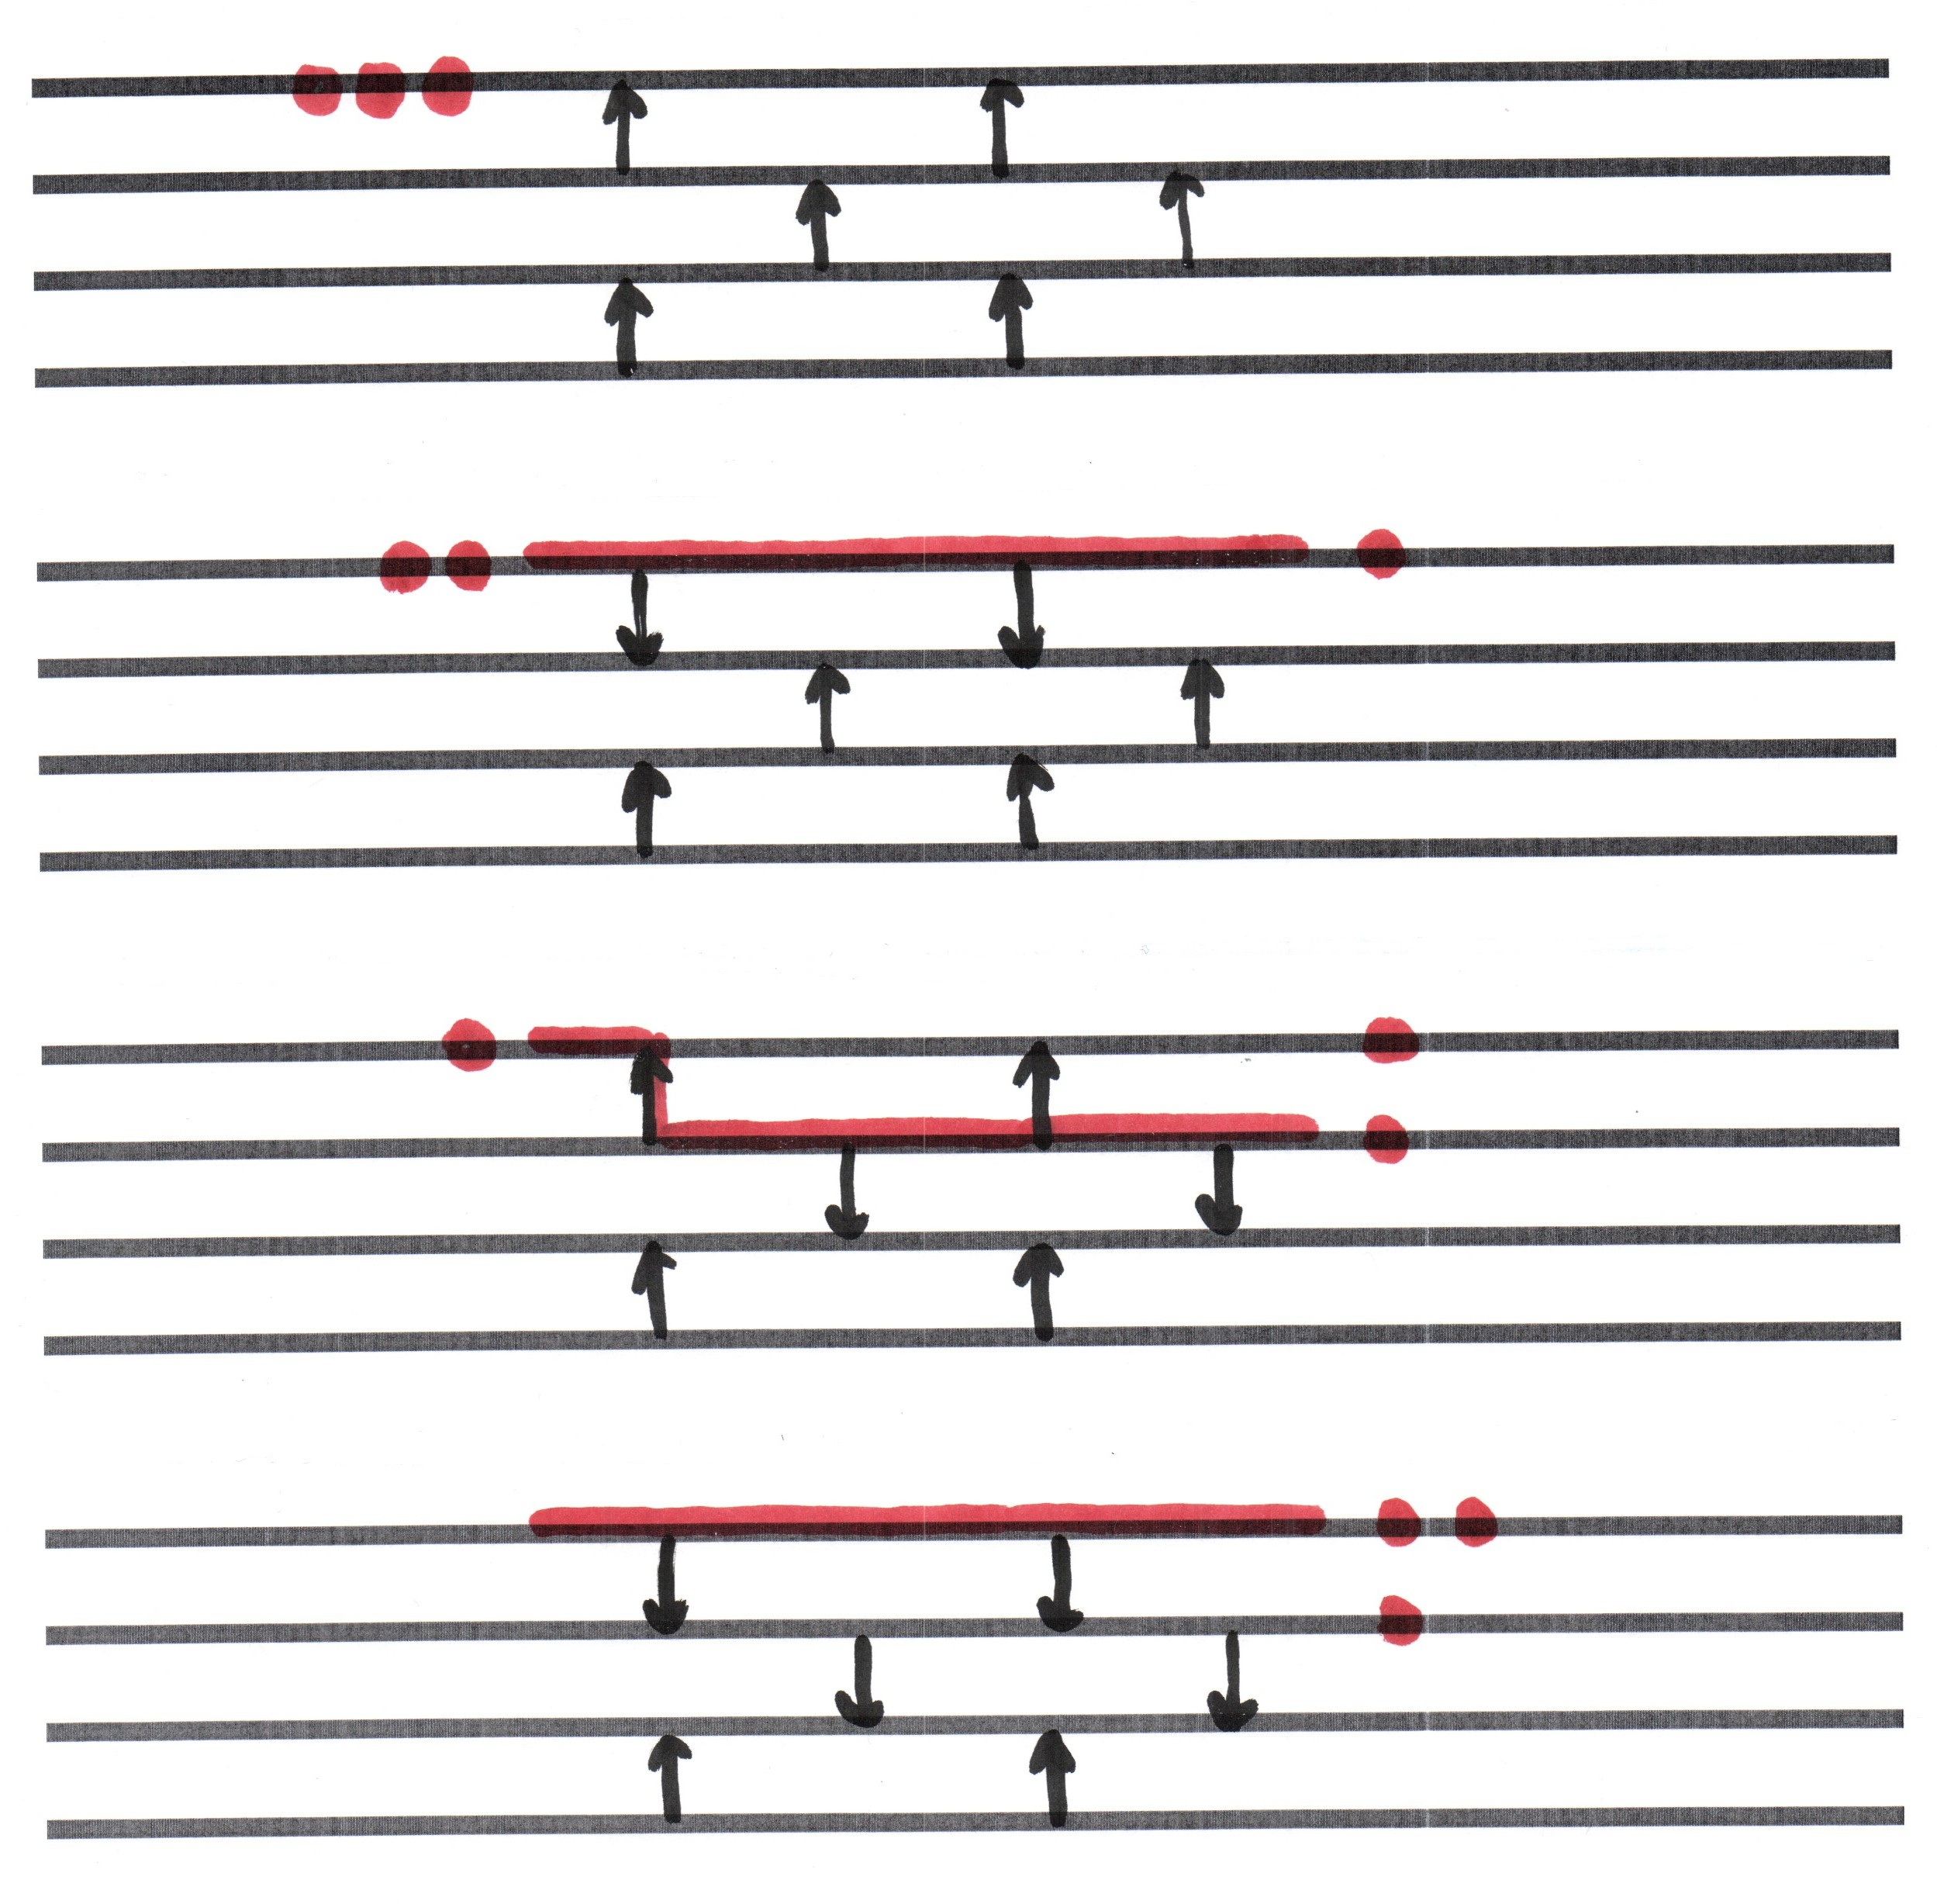
\includegraphics[width=8cm]{oddeven.jpg}\\
\caption{OddEven(4) network is not a counting network}\label{oddeven}
\end{figure}

\subsection{Part (b)}
\noindent\textbf{Proof}:
According to the zero-one theorem, it suffices to show that OddEven($n$) network sorts every length-$n$ binary array of zeros and ones.

Take an arbitrary length-$n$ binary array $A$. Suppose there are $k$ ones in $A$. Let their indices be $\alpha_1<\alpha_2<\cdots<\alpha_k$. For simplicity denote the $i$-th element one (the one on input wire $\alpha_i$) by $1_i$.

First consider $1_1$. If $\alpha_1$ is even, $1_1$ is on the lower wire of a comparator on the first layer (depth $=1$) and compared against a zero. Therefore $1_1$ goes up a level (wire), meanwhile leaving this zero between $1_1$ and $1_2$. Then $1_1$ is compared with all other zeros in front. Each comparator raises $1_1$ by a level. After $\alpha_1-1$ layers (including the first one), $1_1$ is raised to the top wire. It then stays on the top wire. (If there is a tie, our convention is the upper wire stays up.) If $\alpha_1$ is odd and $\alpha_1>1$, $1_1$ is on the upper wire of a comparator on the first layer, after which it remains on wire $\alpha_1$. Starting from the second layer, $1_1$ rises continuously until reaching the top wire. Finally, if $\alpha_1=1$, $1_1$ is always on the top wire.

Then consider $1_2$. Suppose $\alpha_1>1$ (otherwise treat $1_2$ as $1_1$). As is discussed above, after the first rise of $1_1$, there is at least a zero between $1_1$ and $1_2$. Since $1_1$ rises continuously until reaching the top wire, we conclude that after $1_1$ begins to rise, $1_2$ never has the chance to compare with $1_1$ before $1_1$ gets to the top wire. This means that $1_2$ is also continuously compared against the zeros in front of it, so it rises continuously until reaching the second topmost wire.

If $\alpha_2-\alpha_1>1$, $1_2$ begins to rise no later than the second layer just like $1_1$, since initially $1_2$ will not be blocked by $1_1$. If $\alpha_2-\alpha_1=1$, however, $1_1$ may block $1_2$ initially. But once $1_1$ begins to rise it will never block $1_2$ anymore. Since $\alpha_1$ and $\alpha_2$ are of opposite odevity, $1_2$ will begin to rise one layer after $1_1$. Therefore, $1_2$ rises no later than the third layer and continues until reaching the second topmost wire.

Generally, we have the following claim.

~

\noindent\underline{Claim}: If $1_i$ has not reached the $i$-th wire prior to the $(i+1)$-th layer, it rises continuously from this layer until reaching the $i$-th wire.

~

\noindent\underline{Proof of the Claim}: By induction. The base case is examined in detail above. Suppose the claim holds for $i$. There are two cases.

~

\noindent Case 1: $1_i$ has not reached the $i$-th wire prior to the $(i+1)$-th layer.

According to the induction hypothesis, $1_i$ rises on the $(i+1)$-th layer. Then it leaves a zero between $1_i$ and $1_{i+1}$. Since it rises continuously until reaching the $i$-th wire, there is always at least a zero between $1_i$ and $1_{i+1}$, so they do not compare during the rising period. Therefore, if $1_{i+1}$ rises at some point, it will continuously compare with the zeros in front, thus continuously rise until reaching the $(i+1)$-th wire.

If $1_i$ blocks $1_{i+1}$ prior to the $(i+1)$-th layer, $1_i$ and $1_{i+1}$ will be on neighboring wires with opposite odevity at some point. Therefore, $1_{i+1}$ will rise one layer after $1_i$ does. Since $1_i$ rises on the $(i+1)$-th layer, $1_{i+1}$ will rise on the $(i+2)$-th layer. And it will rise continuously until reaching the $(i+1)$-th wire.

If $1_i$ does not block $1_{i+1}$ prior to the $(i+1)$-th layer, it actually never blocks $1_{i+1}$ until reaching the $i$-th wire. Then just like $1_1$, $1_{i+1}$ will rise continuously from no later than the second layer until reaching the $(i+1)$-th wire. Therefore, if it has not reached the $(i+1)$-th wire prior to the $(i+2)$-th layer, it will rise continuously from this layer until doing so.

~

\noindent Case 2: $1_i$ has reached the $i$-th wire prior to the $(i+1)$-th layer.

Prior to the $(i+2)$-th layer, if $1_{i+1}$ is blocked by $1_i$, it means that $1_{i+1}$ has already reached the $(i+1)$-th wire. If $1_{i+1}$ is not blocked by $1_i$, it will continuously rise until being blocked by $1_i$. At this moment, it has reached the $(i+1)$-th wire.

~

Therefore, in both cases, the claim holds for $1_{i+1}$. By induction, the claim is true.

\rightline{\underline{QED}}

~

Since there are $\alpha_i-i$ zeros in front of $1_i$, according to the claim, if $1_i$ has not reached the $i$-th wire prior to the $(i+1)$-th layer, it will need at most $\alpha_i-i$ continuous layers to rise, the first being the $(i+1)$-th layer. Thus it completes all the rises no later than layer No. $(i+1)+(\alpha_i-i)-1=\alpha_i$.

In other words, for all $i\leqslant k$, $1_i$ is sent to its right place within $\alpha_i$ layers. Therefore, to put the length-$n$ binary array $A$ with $k$ ones in order, one needs at most $\alpha_k$ layers. Since the OddEven($n$) network contains $n\geqslant\alpha_k$ layers, we conclude that OddEven($n$) network can sort $A$. Since $A$ is an arbitrary length-$n$ binary array, by the zero-one theorem, OddEven($n$) network is a sorting network. The only requirement for $n$ is $n\geqslant2$, such that comparators can exist in the network.

\section{Monotone Priority Queue}
\subsection{Part (a)}
\begin{enumerate}
\item\textsc{Init}: There is a length-$n$ loop. So the runtime is $O(n)$.
\item\textsc{Delete}: Locating the $i$-th element and assigning a value cost constant time. So the runtime is $O(1)$.
\item\textsc{DeleteMin}: The algorithm loops until it finds the minimum position. So the runtime is $O(n)$.
\end{enumerate}

\subsection{Part (b)}
\noindent\textbf{Description}:
We maintain a pointer $p$ in the priority queue, in front of which no element exists. By ``exists'', I mean ``has value True''.
\begin{enumerate}
\item In \textsc{Init}, after assigning initial values in the loop, set $p$ pointing to the $A[1]$.
%\item In \textsc{Delete}, check if $p$ points to the element being deleted. If so, we need to update the minimum. Loop towards the end of the array until for the first time an element exists (has value True). Redirect $p$ to this element. If no such element exists, set $p$ to NULL.
%\item In \textsc{DeleteMin}, check if $p$ points to NULL. If not, delete the element it points to, then update the minimum just like \textsc{Delete} does. (Loop towards the end of the array until for the first time an element exists. Redirect $p$ to this element. If no such element exists, set $p$ to NULL.)
\item To maintain the $O(1)$ runtime (without amortization) of \textsc{Delete}, we do not change it.
\item In \textsc{DeleteMin}, if $p$ points to NULL, return 0 saying that the priority queue is empty. Otherwise, loop from (the element pointed by) $p$ towards the end of $A$, until we either (1) find the first element $A[i]$ that exists, or (2) find that no element exists.

In case (1), we pop (delete and return the value of) $A[i]$. If $i<n$, set $p$ pointing to $A[i+1]$. Otherwise, set $p$ pointing to NULL. In case (2), we return 0 saying that the priority queue is empty, and set $p$ pointing to NULL.
\end{enumerate}

~

\noindent\textbf{Correctness}:
We prove by induction that at any moment in the algorithm, if $p$ is not NULL, no element before it can exist. It follows that if we start from $p$ and loop towards the end of $A$, the first True element (if any) is the minimum. And if no True element is found, the priority queue is empty.

~

\noindent\underline{Induction Proof}:
At the beginning of the algorithm, $p$ points to $A[1]$. Thus no element before $p$ can exist. Suppose no element before $p$ exists prior to a \textsc{Delete} or a \textsc{DeleteMin} operation. We prove the same is true after this operation.

\textsc{Delete} operation does not move $p$, and it does not change any False to True. Therefore, if no element before $p$ exists prior to a \textsc{Delete}, it is still the case after the \textsc{Delete}.

\textsc{DeleteMin} finds the first True element starting from $p$ and sets it False. Call this element $A[i]$. No element between $p$ and $A[i]$ (both ends included) exists. According to the induction hypothesis, this means that no element upto $A[i]$ (included) exists. When $i<n$, it is legal to set the new $p$ pointing to $A[i+1]$. By the analysis above, no element before $p$ exists after the \textsc{DeleteMin} operation.

By induction, it is proved that if $p$ is not NULL, no element before it can exist.

\rightline{\underline{QED}}

~

From the analysis above, \textsc{DeleteMin} is always deleting the correct minimum. If $p$ is set NULL, it means that we have searched to the end of $A$ without finding any existing element. Therefore, $p$ pointing to NULL indicates an empty priority queue. This proves the correctness of the algorithm.

~

\noindent\textbf{Amortized Runtime Analysis}:
Use aggregate analysis. Notice that $p$ is always moved towards the end of the array. So it is moved at most $n$ steps, each of which costing constant time. Moreover, each element is accessed and deleted only once. So a sequence of \textsc{DeleteMin} operations cost in total $O(n)$ time. Thus the amortized runtime is $O(1)$. Moreover, notice that \textsc{Init} still costs $O(n)$ time and \textsc{Delete} still costs $O(1)$ time.

\section{Infinite Stack}
\subsection{Part (a)}
\noindent In the worst case, $n=\sum_{i=1}^r3^i$, so $S_0$ upto $S_r$ are full. Then if we push one more element, all the previous $n$ elements have to be moved. The worst-case cost is thus $O(n)$.

\subsection{Part (b)}
\noindent\textbf{Proof}:
Consider the stack $S_k$. Suppose the $\alpha$-th push requires elements in $S_k$ to be moved into $S_{k+1}$. The room-making operation creates $|S_k|$ space in $\bigcup_{i=1}^kS_i$. Therefore, in the next $|S_k|$ pushes (including the $\alpha$-th one), $S_k$ will never overflow. We conclude that the elements in $S_k$ need to be transferred to $S_{k+1}$ no more frequently than once every $|S_k|=3^k$ pushes.

As a result, after $n$ pushes, the elements in $S_k$ are moved at most $\lceil n/3^k\rceil$ times, each time the cost being $3^k$. Suppose the largest stack used is $S_r$. Therefore, the total cost is
\begin{equation*}
\sum_{\alpha=1}^nc_\alpha\leqslant\sum_{k=0}^r3^k\lceil n/3^k\rceil<\sum_{k=0}^r(n+3^k)=n(r+1)+\frac{1}{2}(3^{r+1}-1)
\end{equation*}

In order to fill upto $S_r$, we need $n>\sum_{k=0}^{r-1}3^k$, which gives $r<\log_3(2n+1)$. Therefore,
\begin{equation*}
\sum_{\alpha=1}^nc_\alpha<n(r+1)+\frac{1}{2}(3^{r+1}-1)<n\log_3(2n+1)+4n+1=O(n\log n)
\end{equation*}

So the amortized cost is $T=(\sum_{\alpha=1}^nc_\alpha)/n=O(\log n)$.

\subsection{Part (c)}
\noindent\textbf{Proof}:
We first make the following claim, which is proved by induction subsequently.

~

\noindent\underline{Claim}:
The number of elements in $S_k$ where $k>0$ is always a multiple of $3^{k-1}$.

~

\noindent\underline{Proof of the Claim}:
The claim is trivially true for the first step. So the base case holds. Suppose the claim is true after $\alpha$ steps of pushing or popping. If the $(\alpha+1)$-th step is a push operation, there are three cases for any $S_k$.
\begin{enumerate}
\item$S_k$ is unchanged. Then its number of elements is a multiple of $3^{k-1}$ by induction hypothesis.
\item$S_{k-1}$ overflows and $S_k$ can accommodate $3^{k-1}$ elements from $S_{k-1}$ without overflowing. By adding $3^{k-1}$, the number of elements in $S_k$ is still a multiple of $3^{k-1}$.
\item$S_{k-1}$ overflows but $S_k$ cannot accommodate $3^{k-1}$ elements from $S_{k-1}$ without overflowing. It follows that $S_k$ originally had $3^k$ elements. Otherwise, by induction hypothesis, $S_k$ would have at least $3^{k-1}$ room available and would not overflow. Therefore, after this step, $3^k$ elements in $S_k$ will be moved to $S_{k+1}$ (possibly overflowing $S_{k+1}$ and need more stacks to make room), and $3^{k-1}$ elements in $S_{k-1}$ will be moved to $S_k$. So $S_k$ eventually has $3^{k-1}$ elements.
\end{enumerate}

If the $(\alpha+1)$-th step is a pop operation, and suppose the infinite stack is nonempty, there are three cases for any $S_k$.
\begin{enumerate}
\item$S_k$ is unchanged. Then its number of elements is a multiple of $3^{k-1}$ by induction hypothesis.
\item$S_{k-1}$ underflows and $S_k$ can give $3^{k-1}$ elements to $S_{k-1}$ without underflowing. By subtracting $3^{k-1}$, the number of elements in $S_k$ is still a multiple of $3^{k-1}$.
\item$S_{k-1}$ underflows and $S_k$ cannot give $3^{k-1}$ elements to $S_{k-1}$ without underflowing. It follows that $S_k$ originally had no element. Otherwise, by induction hypothesis, $S_k$ would have at least $3^{k-1}$ elements available and would not underflow. Moreover, all stacks smaller than $S_k$ are all empty, otherwise there is no need to borrow elements from $S_k$. Since the infinite stack is nonempty, there must be some $k'>k$, such that $S_{k'}$ is not empty. By induction hypothesis, $S_{k'}$ has at least $3^{k'-1}$ elements. Therefore, starting from $S_{k'-1}$ down to $S_0$, every stack can take enough elements from the triply larger stack to fill itself. Specifically, $S_k$ can take $3^k$ elements from $S_{k+1}$ and give $3^{k-1}$ elements to $S_{k-1}$. So $S_k$ eventually has $2\times 3^{k-1}$ elements.
\end{enumerate}

We see that after the $(\alpha+1)$-th step, in all cases, the number of elements in $S_k$ ends up being a multiple of $3^{k-1}$. This holds for all $k>0$. Therefore by induction, the claim is proved.

\rightline{\underline{QED}}

~

Two corollaries from this claim are as follows. They are already shown in the proof above.

~

\noindent\underline{Corollary}:
If $S_k$ overflows in a push, it will have $3^{k-1}$ elements after this operation.

~

\noindent\underline{Corollary}:
If $S_k$ underflows in a pop, it will have $2\times 3^{k-1}$ elements after this operation.

~

Consider the stack $S_k$ where $k>0$. Suppose a push operation requires elements in $S_k$ to be moved into $S_{k+1}$. According to the first corollary, after room-making, $S_k$ will be filled up by $1/3$. Therefore, in the next $|S_k|/3$ steps, there is no way to push enough elements to overflow $S_k$, or to pop enough elements to underflow $S_k$.

Suppose a pop operation requires $S_k$ to borrow elements from $S_{k+1}$. According to the second corollary, after room-making, $S_k$ will be filled up by $2/3$. Therefore, in the next $|S_k|/3$ steps, there is no way to push enough elements to overflow $S_k$, or to pop enough elements to underflow $S_k$.

It follows that overflow or underflow of $S_k$ happens no more frequently than once every $|S_k|/3=3^{k-1}$ steps. Therefore, after $m$ steps, room-making for $S_k$ is required at most $\lceil m/3^{k-1}\rceil$ times, each time the cost being $3^k$. This also holds for $k=0$. Suppose the largest stack ever used is $S_r$. Therefore, the total cost is
\begin{equation*}
\sum_{\alpha=1}^mc_\alpha\leqslant\sum_{k=0}^r3^k\lceil m/3^{k-1}\rceil<\sum_{k=0}^r(3m+3^k)=3m(r+1)+\frac{1}{2}(3^{r+1}-1)
\end{equation*}

Suppose the maximum number of elements the infinite stack ever had is $n$. Then $n>\sum_{k=0}^{r-1}3^k$, which gives $r<\log_3(2n+1)$. Moreover, $m\geqslant n$. Therefore,
\begin{equation*}
\sum_{\alpha=1}^mc_\alpha<3m(r+1)+\frac{1}{2}(3^{r+1}-1)<3m\log_3(2n+1)+3m+3n+1=O(m\log n)
\end{equation*}

So the amortized cost is $T=(\sum_{\alpha=1}^mc_\alpha)/m=O(\log n)$.

\end{document}
